\documentclass[12pt, twoside]{article}
\documentclass[12pt, twoside]{article}
\usepackage[letterpaper, margin=1in, headsep=0.2in]{geometry}
\setlength{\headheight}{0.6in}
%\usepackage[english]{babel}
\usepackage[utf8]{inputenc}
\usepackage{microtype}
\usepackage{amsmath}
\usepackage{amssymb}
%\usepackage{amsfonts}
\usepackage{siunitx} %units in math. eg 20\milli\meter
\usepackage{yhmath} % for arcs, overparenth command
\usepackage{tikz} %graphics
\usetikzlibrary{quotes, angles}
\usepackage{graphicx} %consider setting \graphicspath{{images/}}
\usepackage{parskip} %no paragraph indent
\usepackage{enumitem}
\usepackage{multicol}
\usepackage{venndiagram}

\usepackage{fancyhdr}
\pagestyle{fancy}
\fancyhf{}
\renewcommand{\headrulewidth}{0pt} % disable the underline of the header
\raggedbottom
\hfuzz=2mm %suppresses overfull box warnings

\usepackage{hyperref}
\usepackage{float}

\fancyhead[LE]{\thepage}
\fancyhead[RO]{\thepage \\ First and last name: \hspace{2.5cm} \,\\ Section: \hspace{2.5cm} \,}
\fancyhead[LO]{BECA/Huson/Geometry: Construction \\* 19 November 2024}

\begin{document}
\subsubsection*{3.7 Trimester Final Exam}
\begin{enumerate}[itemsep=0.5cm]
\item Given $\overline{DEF}$, $DE=3 \frac{1}{3}$, and $EF=1$. Find ${DF}$. \par \bigskip
  \begin{tikzpicture}
    \draw [-, thick] (1,0)--(7,0);
    \draw [fill] (1,0) circle [radius=0.05] node[below]{$D$};
    \draw [fill] (5,0) circle [radius=0.05] node[below]{$E$};
    \draw [fill] (7,0) circle [radius=0.05] node[below]{$F$};
  \end{tikzpicture}  \vspace{2cm}

\item Point $G$ bisects $\overline{FH}$, with $FG=4x-3$, $GH=13$. Find $x$. \par \medskip
  \begin{tikzpicture}
      \draw[fill] (0,0) circle [radius=0.05] node[below]{$F$};
      \draw[-, thick] (0,0)--(8,0);
      \draw[fill] (4,0) circle [radius=0.05] node[below]{$G$};
      \draw[fill] (8,0) circle [radius=0.05] node[below]{$H$};
      \node at (2,0.5) [above]{$4x-3$};
      \node at (6,0.5) [above]{$13$};
      \draw (1.8,-0.2)--(1.9,0.2);
      \draw (2.1,-0.2)--(2.2,0.2);
      \draw (5.8,-0.2)--(5.9,0.2);
      \draw (6.1,-0.2)--(6.2,0.2);
  \end{tikzpicture} \vspace{4cm}

\item The diagram shows $\overline{JKL}$ with $JK=4x+5$, $KL=x+1$, $JL=16$. Find ${x}$.
  \begin{center}
  \begin{tikzpicture}
      \draw [-, thick] (0,0)--(9,0);
      \draw [fill] (0,0) circle [radius=0.05] node[below]{$J$};
      \draw [fill] (7,0) circle [radius=0.05] node[below]{$K$};
      \draw [fill] (9,0) circle [radius=0.05] node[below]{$L$};
      \node at (3.5,0) [above]{$4x+5$};
      \node at (8,0) [above]{$x+1$};
      \draw [<->, dashed] (0,-1)--(9,-1);
      \node at (4.5,-1) [below]{$16$};
  \end{tikzpicture}
  \end{center} \vspace{6cm}


\newpage
\item Bisect the given angle. \vspace{2cm}
  \begin{center}
  \begin{tikzpicture}
    \draw [<->, thick] (80:6)--(0,0)--(20:6);
    \draw [fill] (0,0) circle [radius=0.05] node[below]{$A$};
  \end{tikzpicture}
  \end{center} \vspace{0.5cm}

\item Construct a perpendicular to $\overline{AB}$ though $C$.\\
%\hspace{1cm} Given the line  $l$ and point $P$.
  \vspace{2cm}
  \begin{center}
  \begin{tikzpicture}
    \draw [<->, thick] (0,0)--(11,0)--(6,3)--cycle;
    \draw [fill] (0,0) circle [radius=0.05] node[left]{$A$};
    \draw [fill] (11,0) circle [radius=0.05] node[right]{$B$};
    \draw [fill] (6,3) circle [radius=0.05] node[above right]{$C$};
  \end{tikzpicture}
  \end{center} \vspace{5cm}

\newpage
\item $\triangle ABC$ is shown with vertices $A(-1,2)$, $B(6,1)$, and $C(5,4)$. Reflect the triangle across the $x$-axis. Label the image $\triangle A'B'C'$ on the graph.
  \begin{center}
    \begin{tikzpicture}[scale=0.7]
      \draw [help lines] (-8,-7) grid (8,7);
      \draw [thick, <->] (-8.4,0) -- (8.4,0) node [below right] {$x$};
      \draw [thick, <->] (0,-7.4)--(0,7.4) node [left] {$y$};
      \draw [thick] (-1,2) node[left] {$A$}--
        (6,1) node[right] {$B$}--
        (5,4) node[above right] {$C$}--
        cycle;
    \end{tikzpicture}
    \end{center}


\item A $110^\circ$ counterclockwise rotation centered at $P$ maps triangle $CAT$ onto triangle $DOG$. \\[0.25cm]
Write the letter or letters for each corresponding object. \vspace{0.25cm}
  \begin{multicols}{2}
    \begin{tikzpicture}[scale=1.4, rotate=20]
      \coordinate [label=above left:$D$](A) at (65:2);
      \coordinate [label=below right:$O$](B) at (1, 0);
      \coordinate [label=right:$G$](C) at (15:3.5);
      \draw [thick] (A)--(B)--(C)--cycle;
      \draw [thick, rotate=-110] (65:2) node[right]{$C$}--
      (1,0) node[below left]{$A$}--
      (15:3.5) node[right]{$T$}--cycle;
      \draw [fill] (0,0) circle [radius=0.05] node[left] {$P$};
      \draw [dashed] (0,0) circle [radius=1];
    \end{tikzpicture}
    \begin{enumerate}
      \item $T \rightarrow$ \vspace{1.5cm}
      \item $A \rightarrow$ \vspace{1.5cm}
      \item $\overline{AC} \rightarrow$ \vspace{1.5cm}
    \end{enumerate}
  \end{multicols}

\newpage
\item A translation is applied to $\triangle ABC$ moving it down 2 and to the right 5.
\begin{enumerate}
  \item Write as coordinate pairs the vertices of the image, $\triangle A'B'C'$ \\[0.3cm]
  $A(3,4) \rightarrow$ \\[0.7cm]
  $B(-2,-3) \rightarrow$ \\[0.7cm]
  $C(0,-1) \rightarrow$ \\[0.2cm]
  \item Which triangle is larger, or are they the same size? Justify your answer.
\end{enumerate} \vspace{3cm}


\item A translation maps $D(2,4) \rightarrow D'(-3,4)$. What is the image of $E(5,-5)$ under the same translation? \vspace{2cm}

\item Apply a counterclockwise rotation of $90^\circ$ centered at the origin to $\triangle ABC$. Plot and label the image on the axes below.
  \begin{flushright}
    \begin{tikzpicture}[scale=.48]
      \draw [help lines] (-8,-6) grid (8,8);
      \draw [thick, <->] (-8.4,0) -- (8.4,0) node [right] {$x$};
      \draw [thick, <->] (0,-6.4)--(0,8.4) node [above] {$y$};
      \draw [thick]
        (2,1) node[below left] {$A$}--
        (5,5) node[right] {$B$}--
        (6,2) node[below] {$C$}--
        cycle;
    \end{tikzpicture}
  \end{flushright}

\newpage

\item Which of the following are true with respect to the angle, m$\angle PQR$?
  \begin{multicols}{2}
    \begin{enumerate}
      \item True \quad False \quad It is an acute angle
      \item True \quad False \quad It's measure is $90^\circ$
      \item True \quad False \quad $\overrightarrow{QP} \perp \overrightarrow{QR}$ 
    \end{enumerate}
    \columnbreak
    \begin{tikzpicture}[scale=0.7, rotate=-20]
      \draw[<->, thick] (4,0)--(0,0)--(0,3);
      \draw (0,0)++(0.3,0)--++(0,0.3)--+(-0.3,0);
      \draw[fill] (0,0) circle [radius=0.05] node[below]{$Q$};
      \draw[fill] (0,2) circle [radius=0.05] node[right]{$P$};
      \draw[fill] (3,0) circle [radius=0.05] node[above]{$R$};
    \end{tikzpicture}
  \end{multicols}

\item What is sum of the degree measures of this linear pair, $\angle ABD$ and $\angle CBD$?
  \begin{center}
    \begin{tikzpicture}[scale=.8, rotate=0]
      \draw  [<->, thick] (-3,0)--(3,0);
      \draw[->, thick] (0,0)--(-1, 2) node[below left]{$D$};
      \draw[fill] (-2,0) circle [radius=0.05] node[below]{$A$};
      \draw[fill] (0,0) circle [radius=0.05] node[below]{$B$};
      \draw[fill] (2,0) circle [radius=0.05] node[below]{$C$};
    \end{tikzpicture}
  \end{center}

\item As shown below, two lines intersect making four angles: $\angle 1$, $\angle 2$, $\angle 3$, and $\angle 4$.
  \begin{multicols}{2}  
    \begin{enumerate}
      \item Name a pair of vertical angles. \vspace{1cm}
      \item Given m$\angle 3 = 80^\circ$, write down m$\angle 1$. \vspace{1cm}
      \item Find m$\angle 4$.
    \end{enumerate}
    \begin{tikzpicture}[scale=0.7, rotate=15]
    \draw[<->, thick] (0,-1.5)--(10,1.5);
    \draw[<->, thick] (2,3.5)--(7,-3.5);
    \node at (3,.4){1};
    \node at (6,-.6){3};
    \node at (5,1){2};
    \node at (4,-1){4};
  \end{tikzpicture}
  \end{multicols} \vspace{0.5cm}

\item Given m$\angle BAC = 4x+2$ and m$\angle CAD = 3x+3$, m$\angle BAD=75^\circ$. Find m$\angle BAC$.
  \begin{flushright}
  \begin{tikzpicture}[scale=1]
    \draw[<->, thick] (-10:4)node[above left]{$B$} 
    --(0,0)node[left]{$A$}
    --(-52:5)node[above right]{$C$};
    \draw[->, thick] (0,0)--(-85:4)node[above left]{$D$};
    \node at (2,-1){$4x+2$};
    \node at (1,-2.5){$3x+3$};
  \end{tikzpicture}
  \end{flushright} \vspace{1.5cm}

\newpage
\item Given two parallel lines and a transversal, with alternate interior angles $m\angle 4 = 5x$ and $m\angle 5 = 2x + 40$. Write an equation, then solve for $x$.
  \begin{flushright}
    \begin{tikzpicture}[scale=1]
      \draw [<->, thick] (0,0)--(7,0);
      \draw [<->, thick] (1,2)--(8,2);
      \draw [<->, thick] (5,-1)--(3,3);
      %\draw [<->, thick] (11,-1)--(9,3);
      %\node at (4, 1.7){$1$};
      \node at (5, 2)[below]{$m\angle 4 = 5x$};
      \node at (4, 0)[above left]{$m\angle 5 = 2x + 40$};
      %\node at (10, 0.25){$3$};
    \end{tikzpicture}
    \end{flushright} \vspace{1cm}
    
    \item Given two parallel lines and a transversal, as shown, with m$\angle 8 = 123^\circ$.
  \begin{multicols}{2}
    \begin{enumerate}[itemsep=0.5cm]
      \item What angle is corresponding to $\angle 8$?
      \item What angle is alternate exterior to $\angle 8$?
      \item Find m$\angle 2$ \vspace{1cm}
    \end{enumerate}
    \begin{flushright}
      \begin{tikzpicture}[scale=1,rotate=20]
      \draw [<->, thick] (3.5,2)--(7,2);
      \draw [<->, thick] (2.5,0)--(6,0);
      \draw [<->, thick] (4,-1)--(5.5,3);
      \node at (4.5,0.3) [left]{$5$};
      \node at (4.5,0.3) [right]{$6$};
      \node at (4.3,-0.3) [left]{$7$};
      \node at (4.3,-0.3) [right]{$8$};
      \node at (5.2,2) [above left]{$1$};
      \node at (5.2,2.1) [above right]{$2$};
      \node at (5,2) [below left]{$3$};
      \node at (5.1,2) [below right]{$4$};
    \end{tikzpicture}
  \end{flushright}
  \end{multicols}

\item Given two parallel lines and a transversal, with m$\angle 1 = 3x-10$ and m$\angle 8 = 2x + 32$. \\ Write an equation, then solve for $x$.
\begin{flushright}
  \begin{tikzpicture}[scale=1]
    \draw [<->, thick] (3,2)--(8,2);
    \draw [<->, thick] (2,0)--(7,0);
    \draw [<->, thick] (4,-1)--(5.5,3);
    \node at (4.5,0.3) [left]{$5$};
    \node at (4.5,0.3) [right]{$6$};
    \node at (4.3,-0.3) [left]{$7$};
    \node at (4.3,-0.3) [right]{$8$};
    \node at (5.2,2) [above left]{$1$};
    \node at (5.2,2) [above right]{$2$};
    \node at (5,2) [below left]{$3$};
    \node at (5,2) [below right]{$4$};
  \end{tikzpicture}
\end{flushright}


\newpage
\item A triangle has two angles measuring $81^\circ$ and $52^\circ$. Find the measure of the third angle.
  \begin{flushright}
  \begin{tikzpicture}[scale=1]
    %\draw [->, thick] (0,0)--(5,5);
    \draw [-, thick] (0,0) node[xshift=0.6cm, yshift=0.4cm]{$81^\circ$}--
      (70:4) node[xshift=0.2cm, yshift=-0.7cm]{?}--
      (4.5,0) node[above, xshift=-0.7cm]{$52^\circ$}--cycle;
  \end{tikzpicture}
  \end{flushright} \vspace{1cm}

  \item Given $\triangle RSU$. If $m\angle UST=x$ and $m\angle R=x-80$, and $m\angle U=x-50$. Find $x$.
  \begin{flushright}
  \begin{tikzpicture}[scale=0.8]
    %\draw [->, thick] (0,0)--(5,5);
  \draw [<-, thick] (8,0)--
    (7,0) node[below]{$T$}--
    (0,0) node[below]{$R$}--
    (2.5,3) node[above]{$U$}--
    (5,0) node[below]{$S$};
  \end{tikzpicture}
  \end{flushright} \vspace{2cm}
  
\item Given isosceles $\triangle LMN$ with $\overline{LM} \cong \overline{NM}$. If $m\angle L=2x+20$ and $m\angle N=3x+5$, find $m\angle M$.
\begin{flushright}
\begin{tikzpicture}[scale=0.8]
  %\draw [->, thick] (0,0)--(5,5);
  \draw [-, thick] (0,0) node[below]{$L$}--
    (2.5,3) node[above]{$M$}--
    (5,0) node[below]{$N$}--cycle;
\end{tikzpicture}
\end{flushright} \vspace{3cm}

\newpage

\item \begin{enumerate}
  \item Graph and label $\triangle ABC$ with $A(0,0)$, $B(3,2)$, and $C(3,0)$.
  \begin{center}
    \begin{tikzpicture}%[scale=.635]
      \draw [help lines] (0,0) grid (10,6);
      \draw [thick, ->] (0,0) -- (10.4,0) node [below right] {$x$};
      \draw [thick, ->] (0,0)--(0,6.4) node [left] {$y$};
    \end{tikzpicture}
  \end{center}
  \item Dilate or stretch the triangle by a factor of $k=3$ centered at the origin.\\ $\triangle ABC \rightarrow \triangle A'B'C'$
  \item Find each ratio or fraction. \\[0.5cm]
    $\displaystyle \frac{A'C'}{AC}=$ \hfill
    $\displaystyle \frac{B'C'}{BC}=$ \hfill
    $\displaystyle \frac{A'B'}{AB}=$ \hspace{2cm}
\vspace{1cm}
\end{enumerate}

\item Triangle $ABC$ is dilated with a scale factor of $k=\frac{5}{3}$ centered at $A$, yielding $\triangle ADE$, as shown. Given $AB=9$, $BC=12$, and $AC=15$. \\[0.25cm] Find $AD$, $AE$, and $DE$. \vspace{0.5cm}
  \begin{flushleft}
  \begin{tikzpicture}[scale=0.4]
    \draw [thick]
    (0,0)node[left]{$B$}--
    (8,0)node[above right]{$C$}--
    (2,6)node[left]{$A$}--cycle;
    \draw [thick]
    (0,0)--
    (-1,-3)node[left]{$D$}--
    (11,-3)node[above right]{$E$}--(8,0);
    \node at (4,0)[below]{$12$};
    \node at (5.3, 3)[right]{$15$};
    \node at (0.3, 2.8)[above]{$9$};
  \end{tikzpicture}
  \end{flushleft}


\end{enumerate}
\end{document}